\section{Class 8 - 22/03/21}
We have talked a lot transmission line and how to design them because in the Electromagnetic Compatibility sector it is very important to take in consideration and know everything about noises.\\
Today we are going to talk about antennas.
\subsection*{General info about antennas}
As we have already seen in some exercise, an antenna could be described as a load in a transmission line, where the voltage generator is the one that generates the signal (\cref{fig:tl_antenna}).
\begin{figure}[H]
    \begin{center}
        \begin{circuitikz}
            \draw (0,0)
            to[sV=$V_{g}$] (0,2.5)
            to[R=$R_{g}$, -o] (2,2.5)
            to[short, -o] (7,2.5)
            to[short] (8.5,2.5)
            to[generic=$Z_{antenna}$] (8.5,0)
            to[short, -o](7,0)
            to[short, -o](2,0)
            to[short](0,0)
            ;
            \draw (4.5,0.71)node[label={[font=\Large]above:$Z_0$}] {}
            ;
          \end{circuitikz}     
    \end{center} \caption{Antenna in a transmission line}\label{fig:tl_antenna} 
\end{figure}
In \cref{fig:antennas_example} we can see an example of transmitting and receiving antennas that can be used to propagate information trough open space.
\begin{figure}[H]
    %    \begin{center}
        \centering
        \begin{subfigure}[b]{0.45\textwidth}\centering
            \resizebox{1\textwidth}{!}{%
            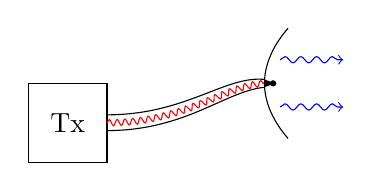
\begin{tikzpicture}[%
                wave/.style={%
                  -,
                  %shorten >=4pt,
                  %shorten <=4pt,
                  decorate,
                  decoration={%
                    snake,
                    segment length=1mm,
                    amplitude=0.4mm,
                    pre length=0pt,
                    post length=0pt,
                  }
                }
              ]
                \draw (0,0) rectangle (1,1) node[pos=.5] {Tx};
                \draw (1,0.6) .. controls (2,0.6) and (2.5,1.1) .. (3,1.05);
                \draw (1,0.4) .. controls (2,0.4) and (2.5,0.9) .. (3,0.95);
                \draw [red,wave] (1,0.5) .. controls (2,0.5) and (2.5,1) .. (3,1);
                \draw [rotate around={-90:(3,1)}] (2.3,1.3) parabola bend (3,1)  (3.7,1.3);
                \fill [black] (3,1.05) -- (3,0.95) -- (3.13,1);
                \fill [black] (3.11,1) circle (0.4mm);
                \draw [blue,wave,->,decorate,
                decoration={%
                  segment length=2mm,
                  amplitude=0.4mm,
                  pre length=0pt,
                  post length=1pt,
                }] (3.2,1.3) -- (4,1.3);
                \draw [blue,wave,->,decorate,
                decoration={%
                  segment length=2mm,
                  amplitude=0.4mm,
                  pre length=0pt,
                  post length=1pt,
                }] (3.2,0.7) -- (4,0.7);
              \end{tikzpicture}}     
        \caption{Transmitter}
    \end{subfigure}%
    \hfill
    \begin{subfigure}[b]{0.45\textwidth}\centering
        \resizebox{1\textwidth}{!}{%
        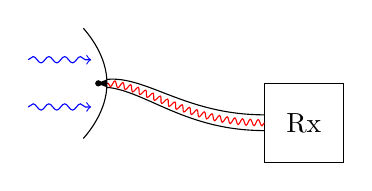
\begin{tikzpicture}[%
            wave/.style={%
              -,
              %shorten >=4pt,
              %shorten <=4pt,
              decorate,
              decoration={%
                snake,
                segment length=1mm,
                amplitude=0.4mm,
                pre length=0pt,
                post length=0pt,
              }
            }
          ]
            \draw (0,0) rectangle (-1,1) node[pos=.5] {Rx};
            \draw (-1,0.6) .. controls (-2,0.6) and (-2.5,1.1) .. (-3,1.05);
            \draw (-1,0.4) .. controls (-2,0.4) and (-2.5,0.9) .. (-3,0.95);
            \draw [red,wave] (-1,0.5) .. controls (-2,0.5) and (-2.5,1) .. (-3,1);
            \draw [rotate around={90:(-3,1)}] (-2.3,1.3) parabola bend (-3,1)  (-3.7,1.3);
            \fill [black] (-3,1.05) -- (-3,0.95) -- (-3.13,1);
            \fill [black] (-3.11,1) circle (0.4mm);
            \draw [blue,wave,->,decorate,
            decoration={%
              segment length=2mm,
              amplitude=0.4mm,
              pre length=0pt,
              post length=1pt,
            }] (-4,1.3) -- (-3.2,1.3);
            \draw [blue,wave,->,decorate,
            decoration={%
              segment length=2mm,
              amplitude=0.4mm,
              pre length=0pt,
              post length=1pt,
            }] (-4,0.7) -- (-3.2,0.7);
          \end{tikzpicture} }   
        \caption{Receiver}
    \end{subfigure}\caption{Antennas example}\label{fig:antennas_example}
\end{figure}
The working principle is very simple and well known: an AC signal is generated by the transmitter circuit, that will be propagated trough a special transmission line which is in fact the antenna in the form of an EM wave.\\
The receiving process is the opposite: The antenna is collecting the EMW colliding to his surface, this will create an AC potential over the wires, that will be converted by the receiving circuit in the original information.\\
This ca sound as an old concept that a lot of people take for granted, but we needed a lot of years and work to come up as a reliable and robust alternative to a wired transmission.
\subsection*{The most simple antenna: the Dipole}
Step by step we are going to create a very simple example of an antenna.\\
First of all, let's consider an open circuited transmission line where some current is moving inside it, as in \cref{fig:TL_dipole1}.
\begin{figure}[H]
    \begin{center}
        \begin{circuitikz}
            \draw (-1,0) to[TL, o-o] (11,0);
            \draw [thick,->] (0,0) -- (3,0); 
            \draw [thick,<-] (3.5,0) -- (6.5,0);
            \draw [thick,->] (7,0) -- (10,0);
            %%  
            \draw (-1,2) to[TL, o-o] (11,2);
            \draw [thick,<-] (0,2) -- (3,2); 
            \draw [thick,->] (3.5,2) -- (6.5,2);
            \draw [thick,<-] (7,2) -- (10,2);
            %%
            \draw [blue!40!black] (-0.15,2.3) parabola bend (1.5,3)  (3.25,2.3);
            \draw [blue!40!black] (3.25,2.3) parabola bend (5,3)  (6.75,2.3);
            \draw [blue!40!black] (6.75,2.3) parabola bend (8.5,3)  (10.25,2.3);
        \end{circuitikz}    
    \end{center} \caption{Transmission line with current oscillation}\label{fig:TL_dipole1} 
\end{figure}
So what happen in this transmission line? The the current (and thus the voltage) is in movement, so we are also moving charge distribution along the line.\\
This charge movement is generating an EMF, so this is an antenna!\\
Not so fast, kid\dots If you look at \cref{fig:TL_dipole1} you can see that this is happening to both of the line, and that is a problem for us, because the EMF generated are opposite one to another. In this case the EMF sum up and cancel each other, and no useful EMF is generated to transmit information outside the line.\\
Now we do something clever: we could separate the end side of the line like in , and let's see what does happen.
\begin{figure}[H]
    \begin{center}
        \resizebox{0.5\textwidth}{!}{%
        \begin{circuitikz}
            \draw (-1,0) to[TL, o-] (8,0)to[TL, -o] (8,-4);
            \draw [thick,->] (0,0) -- (3,0); 
            \draw [thick,<-] (3.5,0) -- (6.5,0);

            \draw [thick,->] (8,-0.6) -- (8,-3);
            %%  
            \draw (-1,2) to[TL, o-] (8,2) to[TL, -o] (8,6);
            \draw [thick,<-] (0,2) -- (3,2); 
            \draw [thick,->] (3.5,2) -- (6.5,2);

            \draw [thick,<-] (8,2.6) -- (8,5);

            \draw [thick,->,blue] (9,5) -- (9,-3);
            %%
        \end{circuitikz}}
    \end{center} \caption{Simple dipole}\label{fig:TL_dipole2} 
\end{figure}
While the first part of the line in \cref{fig:TL_dipole2} does not produce EMF, the second one that we have bent is generating a current distribution in phase and in vertical direction.\\
This does mean that we are moving electric charges along a vertical axe, and so we are generating an EMF! What we have created is a very rudimentary antenna that we call \emph{Dipole}.
\subsubsection*{How i need to build my dipole?}
Now that we have seen the basics, we could be curious to know how to build an appropriate dipole antenna. The physical form it quite straight forward, but how long should our vertical termination be?\\Hertzian 
It depends on my desired current distribution over the antenna: for example if the length of my dipole is $l=\lambda$ (full wave dipole), the current distribution will be able to be distributed 2 times in the total length like in . Why this?\\
Think about you are making a photo at the current distribution when it reach the maximum peak (it is a wave, will reach its peak every half period): at the absolute top and bottom the current will always be zero (it can not go anywhere, because it sees an open circuit).\\
Imagine to travel along a steady wave: you start from 0 and after a quarter of the wavelength you reach a peak of amplitude (i know that this is confusing, just think about the figure of the wave and what you can find every $\frac{\lambda}{4}$). If we travel along the photograph of the "imaginary line" mentioned before, we will see the first peak of the current wave in the half of one conductor (or a quarter of the total antenna length starting from the bottom). At the center of the antenna, the current wave will be 0 again (because we are in the middle of the wavelength, and we started from 0). For the other terminal the situation is exactly the same. This situation can be seen in \cref{fig:Full_wave_antenna}.
In \cref{fig:Half_wave_antenna} you can see the current distribution in an half wave antenna, here the length is $l=\frac{\lambda}{2}$.\\
Similarly to how we have seen the full wave antenna, the current distribution starts from 0 from one node, but now we reach the first amplitude peak on the center of the TL because the total length is now an half of $\lambda$. In this way we have created a pretty capable antenna.\\
The half wave antenna ideally is the best one, because it will behave like a pure resistive load\cite{Antenne_appunti_tlc} (this behavior will be described better during the next lecture, but i can already tell you that it happen if the length is just a little bit shorter than $\frac{lambda}{2}$). Sometimes we need to shrink the length for our application (think that our car should have an antenna $75\si{\centi\metre}$ long), and we can use smaller antennas by adapting the line.
\begin{figure}[H]
    %    \begin{center}
        \centering
        \begin{subfigure}[b]{0.45\textwidth}\centering
            \resizebox{0.1\textheight}{!}{%
            \begin{circuitikz}
                \draw (0,-0.1) to[short, o-] (2,-0.1)
                to[short,line width=1mm] (2,-8);
                \draw (0,0.1) to[short, o-] (2,0.1)
                to[short,line width=1mm] (2,8);
                \draw [blue!40!black,rotate around={-90:(2,0)}] (2,0) parabola bend (6,2.5)  (10,0);
                \draw [blue!40!black,rotate around={90:(2,0)}] (2,0) parabola bend (6,-2.5)  (10,0);
                %rotate around={-90:(3,1)}
            \end{circuitikz}}  
        \caption{Full wave antenna}\label{fig:Full_wave_antenna} 
    \end{subfigure}%
    \hfill
    \begin{subfigure}[b]{0.45\textwidth}\centering
        \resizebox{0.1\textheight}{!}{%
        \begin{circuitikz}
            \draw (0,-0.1) to[short, o-] (2,-0.1)
            to[short,line width=1mm] (2,-8);
            \draw (0,0.1) to[short, o-] (2,0.1)
            to[short,line width=1mm] (2,8);
            \draw [blue!40!black,rotate around={-90:(2,8)}] (2,8) parabola bend (10,11)  (18,8);
            %rotate around={-90:(3,1)}
        \end{circuitikz}} 
        \caption{Half wave antenna}\label{fig:Half_wave_antenna}
    \end{subfigure}\caption{Current distribution in an dipole antenna}
\end{figure}
If we shrink the antenna length, the situation will be similar to the half wave antenna in \cref{fig:Half_wave_antenna}, because the current distribution will not have much space to "place" zero points along the line, and we will always find the peak on the center of the line.\\
Now, if you shrink the antenna a lot, we can assume that the current distribution is the same all over the length ($l<<\lambda$). This is a very appreciated simplification so what we are going to study now on is a very famous (and tiny) \emph{Hertzian Dipole Antenna} with $l=\frac{\lambda}{50}$.
\subsection*{Spherical coordinate}
Attention!! Calculations is going to become more tricky and strange for our antenna (Until now that weren't fancy enough\dots).\\
Since we are dealing with antennas, we should start to think about a way to study the waves trough a tridimensional medium. Here we introduce the Spherical coordinate (probably you already know that).\\
We are in a 3-Dimensional space, but instead collecting the various position of the points with the classical cartesian coordinates $(x,y,z)$, we will use 3 new information:
\begin{itemize}
    \item $\bm{r}$: radial distance $\in (-\infty,+\infty)$
    \item $\bm{\theta}$: azimuthal angle $\in (0,180)$
    \item $\bm{\varphi}$: polar angle $\in (0,360)$
\end{itemize}
It become very clear looking at the plot on \cref{fig:3d_plot}.
\begin{figure}[H]
    \begin{center}
        \begin{tikzpicture}[scale=5,tdplot_main_coords]
            \pgfmathsetmacro{\rvec}{.8}
            \pgfmathsetmacro{\thetavec}{30}
            \pgfmathsetmacro{\phivec}{60}
            \coordinate (O) at (0,0,0);
            \draw[thick,->] (0,0,0) -- (1,0,0) node[anchor=north east]{$x$};
            \draw[thick,->] (0,0,0) -- (0,1,0) node[anchor=north west]{$y$};
            \draw[thick,->] (0,0,0) -- (0,0,1) node[anchor=south]{$z$};
            \tdplotsetcoord{P}{\rvec}{\thetavec}{\phivec}
            \draw[-stealth,color=red!80!black] (O) -- (P) node[above right] {$P$} node[below,midway] {$r$};
            \draw[dashed, color=red!80!black] (O) -- (Pxy);
            \draw[dashed, color=red!80!black] (P) -- (Pxy);
            \tdplotdrawarc{(O)}{0.2}{0}{\phivec}{anchor=north}{$\varphi$}
            \tdplotsetthetaplanecoords{\phivec}
            \tdplotdrawarc[tdplot_rotated_coords]{(0,0,0)}{0.5}{0}%
                {\thetavec}{anchor=south west}{$\theta$}
        \end{tikzpicture}
    \end{center} \caption{3-d plot with Spherical coordinates}\label{fig:3d_plot} 
\end{figure}
It is very simple to go from a coordinate to another (and vice versa), but we are not going to discuss it here.
\subsection*{Hertzian dipole in spherical coordinate}
Going back to ur little antenna, we can describe the EMF on the space with this spherical coordinate:
\begin{equation}
    \phas{E}(r,\theta,\varphi)=\overline{E}_r(r,\theta,\varphi)\hat{r}+\overline{E}_\theta(r,\theta,\varphi)\hat{\theta}+\overline{E}_\varphi(r,\theta,\varphi)\hat{\varphi}
\end{equation}
In \cref{fig:E_in_3d_radial} you can see a nice representation of the dipole in the space coordinate, and the electric field in the spherical coordinates that it generates.
\begin{figure}[H]
    \begin{center}
        \begin{tikzpicture}[scale=5,tdplot_main_coords]
            \pgfmathsetmacro{\rvec}{.7}
            \pgfmathsetmacro{\thetavec}{40}
            \pgfmathsetmacro{\phivec}{60}
            \coordinate (O) at (0,0,0);
            \draw[thick,->] (0,0,0) -- (1,0,0) node[anchor=north east]{$x$};
            \draw[thick,->] (0,0,0) -- (0,1,0) node[anchor=north west]{$y$};
            \draw[thick,->] (0,0,0) -- (0,0,1) node[anchor=south]{$z$};

            \draw[line width=0.7mm, color=blue!50!black]  (0,0,0.3) -- (0,0,0.05) node[left]{Antenna};
            \draw[line width=0.7mm, color=blue!50!black] (0,0,-0.05) -- (0,0,-0.3);

            \tdplotsetcoord{P}{\rvec}{\thetavec}{\phivec}
            \tdplotsetcoord{P2}{\rvec +0.2}{\thetavec}{\phivec}
            \draw[-stealth,color=red!80!black] (P) -- (P2) node[above right] {$\overline{E}(r,\varphi,\theta)$};
            \draw[dashed] (O) -- (P) node[below,midway] {$r$};
            \draw[dashed] (O) -- (Pxy);
            \draw[dashed] (P) -- (Pxy);
            \tdplotdrawarc{(O)}{0.2}{0}{\phivec}{anchor=north}{$\varphi$}
            \tdplotsetthetaplanecoords{\phivec}
            \tdplotdrawarc[tdplot_rotated_coords]{(0,0,0)}{0.5}{0}%
                {\thetavec}{anchor=south west}{$\theta$}
        \end{tikzpicture}
    \end{center} \caption{E vector in Spherical coordinates}\label{fig:E_in_3d_radial} 
\end{figure}
Now we are going to introduce the equation of the various components of the EMF in the spherical space (phasor domain) generated by the Hertzian dipole, but we are not going to demonstrate it.
\begin{equation}\label{eq:EMF_components_in_spherical}
    \begin{cases}
        \overline{E}_r=\eta \, \frac{I_0\, d}{2\pi}\left(\frac{1}{r^2}+\frac{1}{jkr^3}\right)\cos(\theta)e^{\,-jkr}\\[5pt]
        \overline{E}_\theta=\eta\,\frac{I_0\,d}{4\pi}\left(\frac{jk}{r}+\frac{1}{r^2}+\frac{1}{jkr^3}\right)\sin(\theta)e^{\,-jkr}\\[5pt]
        \overline{E}_\varphi=0\\[5pt]
        \overline{H}_r=0\\[5pt]
        \overline{H}_\theta=0\\[5pt]
        \overline{H}_\varphi=\frac{I_0\,d}{4\pi}\left(\frac{jk}{r}+\frac{1}{r^2}\right)\sin(\theta)e^{\,-jkr}\\[5pt]
    \end{cases}
\end{equation}
There is no phasor indicators over the components to simplify a bit the notation.\\
Note that: $\eta =\sqrt{\frac{\mu}{\varepsilon}}$, $k=\frac{\omega}{c}=\omega\sqrt{\mu\varepsilon}$ and $\mu=\frac{2\pi}{\lambda}$.\\
From what you can see in \cref{eq:EMF_components_in_spherical}, when we are far from the antenna we can neglect the components with $\frac{1}{r^2}$ and $\frac{1}{r^3}$ because them will become very small compared to $\frac{1}{r}$. Then we can write the only two remaining components of the EMF:
\begin{equation}\label{eq:EMF_components_in_spherical_2}
\begin{cases}
    \overline{E}_\theta = j\eta \frac{I_0\,d\,k}{4\lambda}\sin(\theta)\frac{e^{\,-jkr}}{r}\\[5pt]
    \overline{H}_\varphi = j\frac{I_0\,d\,k}{2\lambda}\sin(\theta)\frac{e^{\,-jkr}}{r}
\end{cases}
\end{equation}
We have obtained in \cref{eq:EMF_components_in_spherical_2} a very great and simple way to describe the EMF generated by an Hertzian dipole, then we can observe that:
\begin{equation}\label{eq:EMF_components_in_spherical_3}
    \overline{H}=\frac{1}{\eta}\,\hat{k}\times\overline{E} 
\end{equation}
Looking at \cref{eq:EMF_components_in_spherical_3} we can also understand the propagation direction of that wave, because both $\overline{E}$ and $\overline{H}$ are perpendicular to $\overline{k}=k_0\,\hat{r}$, and so the wave is propagating in $\hat{r}$ direction.\\
What does it mean? If you think about the spherical coordinates in \cref{fig:3d_plot}, the $r$ direction is the radial distance from the center, so we can see at the propagation of the field in spherical direction, as can be seen in \cref{fig:Concentric_wavefront}.
\begin{figure}[H]
    \begin{center}
        \tdplotsetmaincoords{45}{135}
        \begin{tikzpicture}[scale=5,tdplot_main_coords]
            \pgfmathsetmacro{\rvec}{.3}
            \pgfmathsetmacro{\rvecc}{.5}
            \pgfmathsetmacro{\rveccc}{.7}
            \pgfmathsetmacro{\thetavec}{20}
            \pgfmathsetmacro{\thetavecc}{50}
            \pgfmathsetmacro{\thetaveccc}{100}
            \pgfmathsetmacro{\phivec}{10}
            \pgfmathsetmacro{\phivecc}{10}
            \pgfmathsetmacro{\phiveccc}{10}
            \shadedraw[tdplot_screen_coords,ball color = white,opacity=0.4] (0,0) circle (\rvec);
            \shadedraw[tdplot_screen_coords,ball color = white,opacity=0.4] (0,0) circle (\rvecc);
            \shadedraw[tdplot_screen_coords,ball color = white,opacity=0.4] (0,0) circle (\rveccc);
            \coordinate (O) at (0,0,0);
            \draw[thick,->] (0,0,0) -- (1,0,0) node[anchor=north east]{$x$};
            \draw[thick,->] (0,0,0) -- (0,1,0) node[anchor=north west]{$y$};
            \draw[thick,->] (0,0,0) -- (0,0,1) node[anchor=south]{$z$};
            
            \tdplotsetcoord{P1}{\rvec}{\thetavec}{\phivec}
            \tdplotsetcoord{P2}{\rvecc}{\thetavecc}{\phivecc}
            \tdplotsetcoord{P3}{\rveccc}{\thetaveccc}{\phiveccc}
            \draw[-stealth,color=red!80!black] (O) -- (P2)  node[below,midway] {$r_2$};
            \draw[-stealth,color=red!80!black] (O) -- (P1)  node[below,midway] {$r_1$};
            \draw[-stealth,color=red!80!black] (O) -- (P3)  node[below,midway] {$r_3$};
            \tdplotsetthetaplanecoords{\phivec}
            \draw[thin,tdplot_rotated_coords] (\rvec,0,0) arc (0:180:\rvec);
            \tdplotsetthetaplanecoords{\phivecc}
            \draw[thin,tdplot_rotated_coords] (\rvecc,0,0) arc (0:180:\rvecc);
            \tdplotsetthetaplanecoords{\phiveccc}
            \draw[thin,tdplot_rotated_coords] (\rveccc,0,0) arc (0:180:\rveccc);
        \end{tikzpicture}
    \end{center} \caption{Concentric propagation of the dipole radiation when we are far from the center}\label{fig:Concentric_wavefront} 
\end{figure}
\subsubsection*{Wavefront of the dipole EMF}
Just to recap, for the planar wave we went from the phasor domain $\phas{E}(z)=\overline{E}_0 e^{\,-j\beta z}$, to the time domain $\overline{E}(t,z)=\overline{E}\cos(\omega t-\beta z)$. Then we "took a photo" of the wave ($\omega t$ is then constant) and tried to see the variation of the $z$ position over the time and we obtained $\frac{\partial z}{\partial t}=\frac{\omega}{\beta}$ (\cref{eq:speed_of_EMF}), so the speed of the wave has the same direction of $z$ and the wavefront are planar.\\
The situation now is not so different, because looking at $E_\theta$ in \cref{eq:EMF_components_in_spherical_2}, it is very similar to $\phas{E}(z)=\overline{E}_0 e^{\,-j\beta z}$, but the exponential is $e^{\,-jkr}$.\\
for everything we have said before, without doing again all the passages, we can play with the similarities between $\overline{E}_\theta$ and $\phas{E}(z)$, and we say that the wavefront could be seen in the space when $kr=constant$, and so the wavefront are placed in concentric spheres because they are propagating in the $r$ direction.\\
Keep in mind that in the $\overline{E}_\theta$ equation there is also $\sin(\theta)$, this mean that we have different amplitudes along all the spherical surface of the wavefront. The last thing to say is that it does not change over $\varphi$, so it is symmetrical over the $z$ axe.
\subsubsection*{Poynting vector and power of an Hertzian dipole}
Another similarity to what we have studied until now is the Poynting vector (\cref{eq:poynting}), so according to its definition we can write:
\begin{equation}
        \overline{S}=\frac{\overline{E}\times\overline{H}^*}{2}=\frac{|\overline{E}|^2}{2\eta}\;\rightarrow\,\left[\si{\frac{\watt}{\metre^2}}\right]
\end{equation}
then we can also describe the power transmitted by the radiation over the sphere with radius $r$:
\begin{align}
    \begin{split}
        P&=\int_{\text{S\tiny{urface}}}\overline{S}\cdot\hat{n}\, d\text{S\tiny{urface}}=\\[5pt]
        &=\int_0^\pi\int_0^{2\pi}\overline{S}\cdot\hat{r}\,\underbrace{r^2\sin(\theta)d\theta}_{d\text{S\tiny{urface}}}\,d\varphi=\\[5pt]
        &=\int_0^{2\pi}d\varphi\int_0^\pi \underbrace{\left(\eta\frac{I_0\,d}{2\lambda}\sin(\theta)\right)^2}_{|E|^2}\,\frac{1}{2\eta}\,\sin(\theta)d\theta
    \end{split}
\end{align}
Then, after some passages, we arrive at the power equation:
\begin{equation}\label{eq:power_of_dipole_far}
    P=\frac{\eta \pi}{3}\,I_0^2\,\left(\frac{d}{\lambda}\right)^2
\end{equation}
This \cref{eq:power_of_dipole_far} is very important because it describes the power that we can transmit to a point far away from the dipole. For the sake of completeness we report the total power transmitted by the dipole (also near field):
\begin{equation}
    P=\frac{\eta \pi}{3}\,I_0^2\,\left(\frac{d}{\lambda}\right)^2-j\eta I_0^2\frac{1}{24\pi^2}\left(\frac{d}{\lambda}\right)^2\left(\frac{\lambda}{r}\right)^3
\end{equation}
So if we are more near to the transmitting dipole, we well see also a reactive power, that could not see if i move away.
\subsection*{More general antennas parameters}
We finish to talk about hertzian dipoles, and now we are starting to talk about some useful parameters that we can find in all kind of antennas (valid also for the dipole).
\subsection*{Generalization of the $\overline{E}$ and $\overline{H}$ of an antenna}
Until now we skipped a lot of passages, and we obtained the equation of $\overline{E}$ and $\overline{H}$ for the Hertzian dipole when we are far from the antenna that you can see in \cref{eq:EMF_components_in_spherical_2}\dots And now we are going to do the same thing for a general antenna too LOL (if you want to go into details, i can suggest you to look at the notes of Prof. Cucinotta from Unipr\cite{Appunti_unipr}).
We now need to introduce the equivalent moment of an antenna, that for the Hertzian dipole is:
\begin{equation}
    \overline{M}=I_0 \, d \, \hat{z}
\end{equation}
You can notice that it is essentially it is the magnetic moment generated by our antenna (more info of that equivalent momentum in \cite{Ellingson2020Radiation}).\\
The trick that we will use to generalize what we are talking about is that we can thing at a random antenna like a lot of little Hertzian dipole, one near the other, and thus we can see them like a lot of little magnetic momentum that generates the field. If you look closer at \cref{eq:EMF_components_in_spherical_2}, you can find this moment as $|M|=I_0\,d$\\
Then, for a generic source with volume volume $V$ the magnetic moment is:
\begin{equation}
    \overline{M}=\int_V\overline{j}_i\,\overline{r^\prime}\,e^{\,jk\overline{r^\prime}\cdot \hat{r}}\, dV
\end{equation}
Where:
\begin{itemize}
    \item $\bm{\overline{j}_i}$ is the volumetric current density.
    \item $\bm{k=\omega\sqrt{\mu\varepsilon}}$ is the module of the wave vector (but we already know that).
    \item $\bm{\overline{r^\prime}}$ is the vector position of all the points that constitute the source.
\end{itemize}
Now we can finally introduce the generalized $E_\theta$ and $H_\varphi$ components for the far distances:
\begin{equation}\label{eq:EMF_components_in_spherical_generalized1}
    \begin{cases}
        \overline{E}_\theta = j\eta \frac{M}{2\lambda}\sin(\theta)\frac{e^{\,-jkr}}{r}\\[5pt]
        \overline{H}_\varphi = j\frac{M}{2\lambda}\sin(\theta)\frac{e^{\,-jkr}}{r}
    \end{cases}
\end{equation}
Unluckily that is not all, because we have only described 2 component of our field.\\
So, we now can introduce the electric field emitted by a generalized antenna with magnetic moment $\overline{M}$
\begin{equation}\label{eq:electric_field_antenna1}
    \overline{E}(r,\theta,\varphi)=\underbrace{j\eta\frac{M(\theta,\varphi)}{2\lambda}\sin(\theta)}_{\theta,\varphi}\underbrace{\frac{e^{\,-jkr}}{r}\hat{\theta}}_r
\end{equation}
In \cref{eq:electric_field_antenna1} we can note that one part is only dependent on $\theta$ and $\varphi$, so we can summarize that with:
\begin{equation}\label{eq:electric_field_antenna_theta_phi}
    \overline{E}(\theta,\varphi)=j\eta\frac{|M(\theta,\varphi)|}{2\lambda}\sin(\theta)
\end{equation}
The \cref{eq:electric_field_antenna_theta_phi} will become very useful to describe our equation because it simplify a lot the notation.\\
We can then exploit \cref{eq:electric_field_antenna_theta_phi} to write the equation of the electric and magnetic field emitted by a generalized antenna:
\begin{equation}\label{eq:electric_field_antenna_generalized}
    \begin{cases}
        \overline{E}(r,\theta,\varphi) =  \overline{E}(\theta,\varphi)\frac{e^{\,-jkr}}{r}\hat{\theta}\\
        \overline{H}(r,\theta,\varphi) = \frac{e^{\,-jkr}}{\eta r} \overline{E}(\theta,\varphi)\hat{\varphi}
    \end{cases}
\end{equation}
\subsubsection*{Poynting vector for general antenna}
Starting from \cref{eq:electric_field_antenna_generalized}, the calculation of the poynting vector is very straight forward:
\begin{equation}
        \overline{S}=\frac{1}{2}\overline{E}\times\overline{H}=\frac{|\overline{E}(\theta,\varphi)|^2}{2\eta r^2}\hat{r}
\end{equation}
\subsubsection*{Power irradiated by a general antenna}
Before we have seen the power irradiated by an Hertzian dipole antenna, now we will be more general. We remember that we can compute the irradiated power by an antenna as the flux of the poynting vector trough a spherical surface with radius $r$:
\begin{align}
    \begin{split}
        P_a&=\int_{\text{S\tiny{urface}}}\frac{|\overline{E}(\omega,\varphi)|^2}{2\eta r^2}\,d\text{S\tiny{urface}}=\\[5pt]
        &=\int_0^{2\pi}\int_0^\pi \frac{|\overline{E}(\theta,\varphi)|^2}{2\eta\cancel{r^2}}\sin(\theta)\cancel{r^2}\,d\theta\,d\varphi
    \end{split}
\end{align}
Now we can introduce the well known solid angle, so we are able to merge the 2 integrals in only one:
\begin{equation}\label{eq:antenna_power}
    P_a=\int_0^{4\pi}\frac{|\overline{E}(\theta,\varphi)|^2}{2\eta}\,d\Omega=\int_0^{4\pi}I_r(\theta,\varphi)\,d\Omega
\end{equation}
\subsubsection*{intensity of radiation}
Here in \cref{eq:antenna_power} we have introduced the intensity of radiation $I_r(\theta,\varphi)$:
\begin{equation}\label{eq:radiation_intensity}
    I_r(\theta,\varphi)=\frac{|\overline{E}(\theta,\varphi)|^2}{2\eta}=|\overline{S}(r,\theta,\varphi)|r^2
\end{equation}
The intensity of radiation is very interesting for us, because it will be helpful to describe its directivity.
\subsubsection*{Isotropic antenna}
Now let's focus on our antenna, and think about we have an antenna that is very good at spreading the radiation everywhere in the space, and it will be called \emph{ISOTROPIC ANTENNA}. As we have said, the radiation intensity should be equal everywhere, so it does not vary on $\theta$ and $\varphi$ ($I_r(\theta,\varphi)=I_r^0$). The power of an isotropic antenna is:
\begin{equation}\label{eq:power_isotropic_antenna}
    P_a^{iso}=\int_0^{4\pi}I^0_r\,d\Omega=I^0_r\,4\pi
\end{equation}
\subsubsection*{Normalized intensity of radiation}
Another important value to introduce now is the \emph{intensity of radiation} $i_r$, that is defined as the ratio between the intensity of radiation of one point, times the maximum value that the intensity of radiation of the same antenna could reach.
\begin{equation}
    i_r(\theta,\varphi)=\frac{I_r(\theta,\varphi)}{I_r^{max}}
\end{equation}
Note that for the isotropic antennas $i_r(\theta,\varphi)=1 \forall \theta,\varphi$
\subsubsection*{Radiation Function}
We introduce here the \emph{radiation function}, that is the square root of the normalized intensity of radiation:
\begin{equation}
    f(\theta,\varphi)=\sqrt{i_r(\theta,\varphi)}
\end{equation}
This function is what will describe the propagation of the antenna on the space
\subsubsection*{Radiation Pattern}
The radiation pattern is the plot in 2 or 3 dimension of the radiation function $f(\theta,\varphi)$, Here i decided to plot in \cref{fig:radiation_function} an approximation of a classic radiation pattern in 2-d axe, where you can find:
\begin{itemize}
    \item \textbf{max}: the point where you can spot the maximum value of the radiation intensity
    \item \textbf{main lobe}: actually the main and the longest lobe, here you can find the max value
    \item \textbf{lateral lobes}
    \item \textbf{back lobes}: the lobes that usually are on the back of the antenna, them are the smallest
\end{itemize}
\begin{figure}[H]
    \begin{center}
        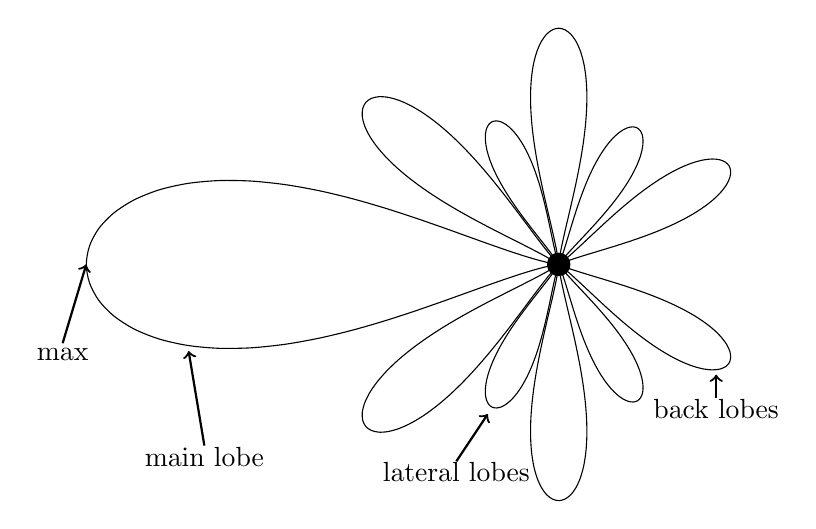
\begin{tikzpicture}
            \draw plot[variable=\t,domain=0:360,smooth,samples=51] 
             ({180+18*sin(\t)}:{6*pow(sin(\t/2),3)});

            \draw plot[variable=\t,domain=0:360,smooth,samples=51] 
             ({220+12*sin(\t)}:{3.2*pow(sin(\t/2),3)});
             \draw plot[variable=\t,domain=0:360,smooth,samples=51] 
             ({140+12*sin(\t)}:{3.2*pow(sin(\t/2),3)});

             \draw plot[variable=\t,domain=0:360,smooth,samples=51] 
             ({115+12*sin(\t)}:{2*pow(sin(\t/2),3)});
             \draw plot[variable=\t,domain=0:360,smooth,samples=51] 
             ({245+12*sin(\t)}:{2*pow(sin(\t/2),3)});

             \draw plot[variable=\t,domain=0:360,smooth,samples=51] 
             ({90+12*sin(\t)}:{3*pow(sin(\t/2),3)});
             \draw plot[variable=\t,domain=0:360,smooth,samples=51] 
             ({270+12*sin(\t)}:{3*pow(sin(\t/2),3)});

             \draw plot[variable=\t,domain=0:360,smooth,samples=51] 
             ({30+12*sin(\t)}:{2.5*pow(sin(\t/2),3)});
             \draw plot[variable=\t,domain=0:360,smooth,samples=51] 
             ({-30+12*sin(\t)}:{2.5*pow(sin(\t/2),3)});

             \draw plot[variable=\t,domain=0:360,smooth,samples=51] 
             ({60+12*sin(\t)}:{2*pow(sin(\t/2),3)});
             \draw plot[variable=\t,domain=0:360,smooth,samples=51] 
             ({-60+12*sin(\t)}:{2*pow(sin(\t/2),3)});

            \node[circle,fill,inner sep=3pt]{};
            
            \draw[thick,<-]  (-4.7,-1.1) -- (-4.5,-2.3) node[yshift=-0.4em]{main lobe};
            \draw[thick,<-]  (-6,0) -- (-6.3,-1) node[yshift=-0.4em]{max};
            \draw[thick,<-]  (-0.9,-1.9) -- (-1.3,-2.5) node[yshift=-0.4em]{lateral lobes};
            \draw[thick,<-]  (2,-1.4) -- (2,-1.7) node[yshift=-0.4em]{back lobes};
           \end{tikzpicture}
    \end{center} \caption{Radiation pattern of a general antenna}\label{fig:radiation_function} 
\end{figure}
\subsubsection*{HPBW: Half-Power Beam Width}
Looking at the radiation pattern in \cref{fig:radiation_function}, we can introduce a few more parameters that will help us to describe the radiation, like the \emph{Half-Power Beam Width}.\\
The HPBW is the angle measured on the main lobe, in which the magnitude of the radiation pattern decreases by 50\% (or -3dB) from the peak of the main beam. It is in fact the area where most of the power is radiated.\\
Maybe it is more clear when you look at the picture in \cref{fig:beam_width_2d}.\\
It could be measured by targeting the two half power point, then the angle between those two is the HPBW.\\
Usually we can find more than one HPBW, because we can choose more than one orthogonal with which i can cut and study my radiation.
\begin{figure}[H]
    \begin{center}
        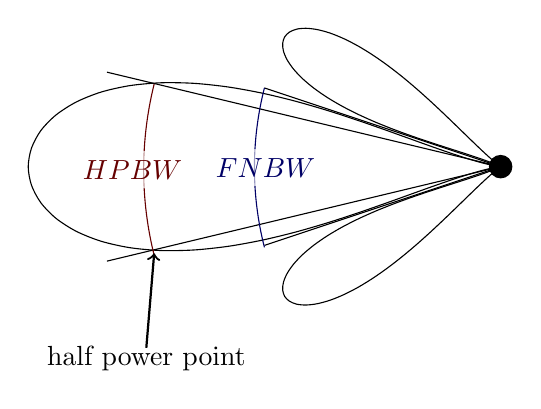
\begin{tikzpicture}
            \draw plot[variable=\t,domain=0:360,smooth,samples=51] 
             ({180+18*sin(\t)}:{6*pow(sin(\t/2),3)});

            \draw plot[variable=\t,domain=0:360,smooth,samples=51] 
             ({211+12*sin(\t)}:{3.2*pow(sin(\t/2),3)});
             \draw plot[variable=\t,domain=0:360,smooth,samples=51] 
             ({149+12*sin(\t)}:{3.2*pow(sin(\t/2),3)});

             \node[circle,fill,inner sep=3pt]{};


             \draw[thin]  (0,0) -- (-5,-1.2);
             \draw[thin]  (0,0) -- (-5,1.2);
             \draw[red!40!black] (-4.4,1.05) arc (166:194:4.5) node[midway,xshift=-0.4em,fill=white,text opacity=1,fill opacity=0.6] {$HPBW$};

             \draw[thin]  (0,0) -- (-3,-1);
             \draw[thin]  (0,0) -- (-3,1);
             \draw[blue!40!black] (-3,1) arc (165.7:194.3:4.1)node[midway,xshift=0.4em,fill=white,text opacity=1,fill opacity=0.6] {$FNBW$};


             \draw[thick,<-]  (-4.4,-1.1) -- (-4.5,-2.3) node[yshift=-0.4em]{half power point};
           \end{tikzpicture}
    \end{center} \caption{HPBW and FNBW in the antenna Radiation pattern}\label{fig:beam_width_2d} 
\end{figure}
\subsubsection*{FNBW: First Null Beam Width}
The \emph{First Null Beam Width} is another interesting angle, used to determine the directivity of the antenna, it is defined as the angular span between the first pattern nulls adjacent to the main lobe. Again, maybe it is better to see it in \cref{fig:beam_width_2d}, but if you get rid of the direction on that plane, you can obtain a simpler graph where the FNBW and the HPBW becomes very clear, that you can see in \cref{fig:antenna_radiation_flat}.

\begin{figure}[H]
    \begin{center}
        \resizebox{0.7\textwidth}{!}{%
        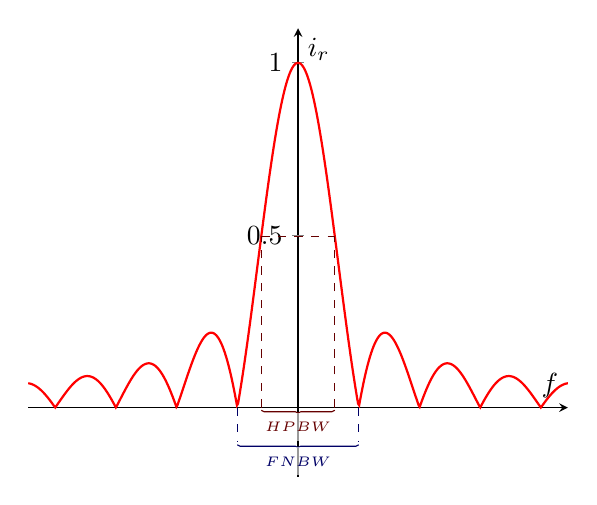
\begin{tikzpicture}
            \begin{axis}[
                axis lines = center,
                xticklabels=none,
                yticklabels=none,
                xtick=\empty,ytick=\empty,
                xlabel = $f$,
                ylabel = {$i_r$},
                scale=1,
                extra y ticks={1,0.5},
                ymax=1.1,
                ymin=-0.2
            ]
            \addplot [
                domain=-8:8,
                samples=500, 
                color=red,
                thick
            ]
            {abs(sin(100*x)/(x*pi/1.8))};
            \addplot [mark=none,dashed,thin,red!40!black] coordinates {(1.09,0) (1.09,{abs(sin(100* 1.09)/(1.09 *pi/1.8))})};
            \addplot [mark=none,dashed,thin,red!40!black] coordinates {(-1.09,0) (-1.09,{abs(sin(100* 1.09)/(1.09 *pi/1.8))})};
            \addplot [mark=none,dashed,thin,red!40!black] coordinates {(-1.09,{abs(sin(100* 1.09)/(1.09 *pi/1.8))}) (1.09,{abs(sin(100* 1.09)/(1.09 *pi/1.8))})};
            \draw [decorate,decoration={brace,amplitude=1pt,raise=1pt},yshift=0pt,red!40!black]
            (1.09,0) -- (-1.09,0) node [midway,fill=white,text opacity=1,fill opacity=0.6,yshift=-0.7em] {\tiny$HPBW$};

            \addplot [mark=none,dashed,thin,blue!40!black] coordinates {(1.8,0) (1.8,-0.1)};
            \addplot [mark=none,dashed,thin,blue!40!black] coordinates {(-1.8,0) (-1.8,-0.1)};

            \draw [decorate,decoration={brace,amplitude=1pt,raise=1pt},yshift=0pt,blue!40!black]
            (1.8,-0.1) -- (-1.8,-0.1) node [midway,fill=white,text opacity=1,fill opacity=0.6,yshift=-0.7em] {\tiny$FNBW$};

            \end{axis}
        \end{tikzpicture}}
    \end{center} \caption{Antenna radiation Pattern in a simplified flat plain}\label{fig:antenna_radiation_flat} 
\end{figure}
\subsubsection*{Directivity}
As you may have already thought, the direction of the beam waves of an antenna is very important! So we introduce now the \emph{directivity} $D$, that is a parameter that in fact condensate everything that we could say about the direction of the beams by directly comparing our antenna with an ideal isotropic antenna (the isotropic antenna is the one that emits in all the directions, so is the worst possible).\\
(maximum) Directivity is defined by the ratio between the maximum value of radiation intensity ($I_r^{max}$) of my antenna, over the radiation intensity of an isotropic antenna ($I_r^0$) which emit the same total power.
\begin{equation}
    D_{max}=\frac{I_r^{max}}{I_r^0}
\end{equation}
Note that this is the maximum directivity, the directivity definition depends on the point in which we measure the intensity of radiation $I_a(\theta,\varphi)$
From \cref{eq:power_isotropic_antenna} we can give another definition of directivity:

\begin{align}\label{eq:directivity2}
    \begin{split}
        D_{max}&=\frac{4\pi\,I_r^{max}}{P_a^{iso}}=\frac{4\pi\,I_r^{max}}{P_a}=\\[5pt]
        &=\frac{4\pi\,I_r^{max}}{\int_0^{4\pi}I_r(\theta,\varphi)\,d\Omega}=\\[5pt]
        &=\frac{1}{\frac{1}{4\pi}\int_0^{4\pi}\frac{I_r(\theta,\varphi)}{I_r^{max}}\,d\Omega}=\\[5pt]
        &=\frac{1}{\frac{1}{4\pi}\int_0^{4\pi}i_r\,d\Omega}
    \end{split}
\end{align}
For this new directivity definition in \cref{eq:directivity2} the numerator is the maximum value of F, and the denominator just represents the "average power radiated over all directions".
To sum up: if my directivity is lower than another antenna, this mean that i will need more power to irradiate the same beam in that specific direction, so having a high $D$ value is very appreciated. In \cref{fig:different_radiation_pattern} you can see an example of two antennas with different directivity, where the "blue" antenna has an higher value of $D$.
\begin{figure}[H]
\begin{center}
    \resizebox{0.6\textwidth}{!}{%
    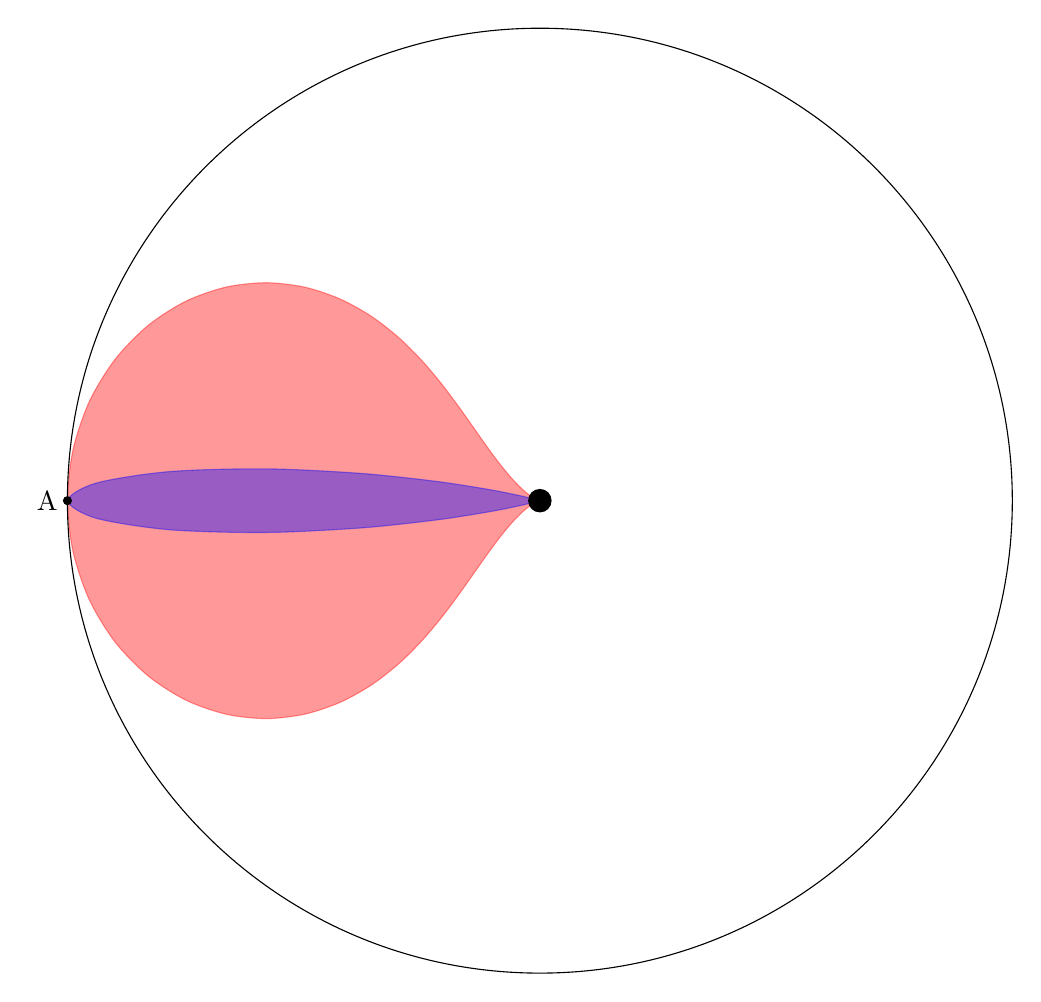
\begin{tikzpicture}
        \draw [fill,red,opacity=0.4] plot[variable=\t,domain=0:360,smooth,samples=51] 
         ({180+50*sin(\t)}:{6*pow(sin(\t/2),3)});

        \draw [fill,blue,opacity=0.4] plot[variable=\t,domain=0:360,smooth,samples=51] 
         ({180+18*sin(\t)}:{6*pow(sin(\t/2),30)});

        \node[circle,fill,inner sep=3pt]{};
        
        \draw[thin] (0,0) circle (6cm);
        \path[draw=black,fill=black] (-6,0) circle (0.05cm) node[left]{A};
       \end{tikzpicture}}
\end{center} \caption{Different Radiation pattern}\label{fig:different_radiation_pattern} 
\end{figure}
\subsubsection*{Efficiency}
Another parameter is the \emph{efficiency}, that measures the amount of power loss by the antenna. It is defined by the ratio between the power emitted by the antenna, over the total power absorbed:
\begin{equation}\label{eq:atenna_efficency}
    \delta=\frac{P_a}{P_{input}}=\frac{P_a}{P_a+P_{loss}}
\end{equation}
\subsubsection*{Effective area}
Until now we have talked a lot about the physical dimension of an antenna, so it is not a surprise if this is a very important parameter.\\
If you think about an antenna, it is clear that the area has an important role for the capacity of receiving radio waves, but even more important is the \emph{effective area}, that is defined as:
\begin{equation}\label{eq:effective_area}
    A_{eff}=\frac{P_r}{\frac{|\overline{E}|^2}{2\eta}}
\end{equation}
Also known as antenna aperture, it is a measure of how effective an antenna is at receiving the power of electromagnetic radiation, and in fact it is the ratio between the power received by the antenna over the poynting vector of the field.\\
To simplify a bit the notation, we define $p$ be the power density of the plane wave (poynting vector of course) and we can easily see how the received power could be obtained:
\begin{equation}\label{eq:effective_area2}
    P_r=p\,A_{eff}
\end{equation}
Please be aware that the definition that we gave in \cref{eq:effective_area} is only true under particular assumption:
\begin{itemize}
    \item \textbf{Same direction} between the antenna and the Beam.
    \item \textbf{Completely matching} between the antenna and the receiver circuit.
    \item \textbf{Same polarization} Between transmitter and receiver.
\end{itemize}
Of course the effective area can be linked to the geometric area by a very simple relation:
\begin{equation}
    A_{eff}=\varepsilon_{ap} A_{geom}
\end{equation}
Where $\varepsilon_{ap}$ is the efficiency of the aperture.
There is also another way to see the effective area, but you will see it later (\cref{eq:true_for_every_antenna})
\subsubsection*{Effective length}
Won't Somebody Please Think of the dipole?? \footnotesize{i hope you got the cit\dots} \\
Anyway, if we deal with a dipole antenna we can introduce the \emph{It is defined as the ratio of the induced voltage to the incident field} $\overline{h}(\theta,\varphi)$, that is defined as the ratio of the induced voltage ($\overline{V}_a$) to the incident field($\overline{E}$):
\begin{equation}
    \overline{h}(\theta,\varphi)=\frac{\overline{V}_a(\theta,\varphi)}{\overline{E}(\theta,\varphi)}
\end{equation}
\subsection*{Circuital representation of an antenna}
Of course, as we said various time before, our antenna could be represented like a load on my transmission line (as we have seen before in \cref{fig:tl_antenna}).\\
Now we are going a little bit more in depth, starting by looking at the impedance of the antenna that can be seen as three different impedances, as you can see in \cref{fig:impedance_antenna}, we will have that $Z_a=R_{loss}+R_{in}+jX_a$ 
\begin{figure}[H]
    \begin{center}
        \resizebox{!}{0.25\textheight}{%
        \begin{circuitikz}
            \draw (0,0)
            to[short,o-](3,0)
            to[generic=$X_{a}$](3,2)
            to[R=$R_{in}$](3,4)
            to[R=$R_{loss}$](3,6)
            to[short,-o](0,6)
            ;
            \draw [decorate,decoration={brace,amplitude=5pt,raise=1pt},yshift=0pt,blue!40!black]
            (3.5,6) -- (3.5,0);
            \draw (4.3,6) 
            to[generic=$Z_{a}$,o-o](4.3,0);
          \end{circuitikz}}  
    \end{center} \caption{Impedance components of an antenna}\label{fig:impedance_antenna} 
\end{figure}
\begin{itemize}
    \item $\bf{R_{loss}}$ Represents the losses inside the physical antenna.
    \item $\bf{R_{in}}$ Represent the power that the antenna is able to irradiate during its operation.
    \item $\bf{X_{a}}$ Reactance of the antenna (usually we would like to be compensate it trough adaption).
\end{itemize}
Then we can give new definition to the power loss and the emitted power, that were used to define the antenna efficiency parameter (\cref{eq:atenna_efficency}):
\begin{align}\label{eq:emitted_power2}
    \begin{split}
        &P_a=\frac{1}{2}\,R_{in}|I|^2\\[5pt]
        &P_{loss}=\frac{1}{2}\,R_{loss}|I|^2
    \end{split}
\end{align}
Then the efficiency of an antenna becomes:
\begin{equation}
    \delta =\frac{R_{in}}{R_{in}+R_{loss}}
\end{equation}
What we have just said is also true for a receiving antenna, but in this case the antenna becomes the generator of the TL, and so we need to add a voltage geneator on the bottom, as you can see in \cref{fig:impedance_antenna_receiving}:
\begin{figure}[H]
    \begin{center}
        \resizebox{!}{0.25\textheight}{%
        \begin{circuitikz}
            \draw (0,-2)
            to[short,o-](3,-2)
            to[sV=$V_{a}$](3,0)
            to[generic=$X_{a}$](3,2)
            to[R=$R_{in}$](3,4)
            to[R=$R_{loss}$](3,6)
            to[short,-o](0,6)
            ;
          \end{circuitikz}}  
    \end{center} \caption{Impedance components of a receiving antenna}\label{fig:impedance_antenna_receiving} 
\end{figure}